\section{Durchführung}
\label{sec:Durchführung}
Eine schematische Darstellung des Versuchsaufbaus ist in Abbildung \ref{fig:Aufbau} zu finden.\\
Der Rezipient wird zunächst mit einer Drehschieber-Vakuumpumpe evakuiert um dann mit Helium gefüllt zu werden.
Dies hat den Vorteil, dass Helium eine
geringere Kondensationstemperatur hat, als der zum kühlen benutzte Stickstoff. So ist sichergestellt, dass sich
keine Flüssigkeiten im Rezipienten bildet.\\
Das Dewargefäß wird mit flüssigem Stickstoff gefüllt und der Reziepient so auf ungefähr 80\,K abzukühlen. Dabei ist darauf
zu achten, dass die Pt-100-Widerstände für die Probe und das Gefäß maximal einen Unterschied von einem $\upOmega$ anzeigen.\\
Ist die Probe abgekühlt wird der Reziepient wieder evakuiert um Konvektion zwischen Probe und Gefäß zu vermeiden.\\
Die Messung wird gestartet indem die Stromversorgung der Heizspulen um Probe und Gefäß eingeschaltet werden. Die Spule für
die Probe wird dabei mit einer konstanten Stromstärke von 150\,mA betrieben. Die Stromstärke der Spule des Gefäßes wird
während des Versuches variiert um sicherzustellen das sich die Probe und das Gefäß gleichmäßig aufheizen um Energieverluste
durch Wärmestrahlung zu unterdrücken.\\
Es werden alle 5 Minuten die Werte der beiden Pt-100-Wiederstände sowie Stromstärke und Spannung an beiden Spannungsgeräten
abgelesen.
\begin{figure}
  \centering
  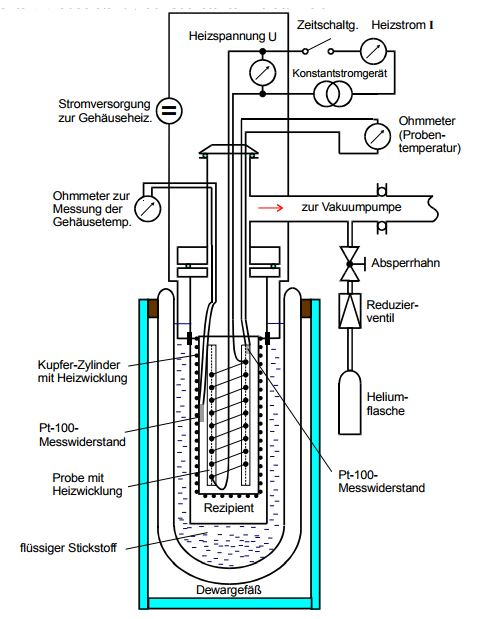
\includegraphics[width=0.6\textwidth]{pics/Aufbau.JPG}
  \caption{Schematische Darstellung des Versuchsaufbaus \cite{Anleitung}.}
  \label{fig:Aufbau}
\end{figure}
